\documentclass[10pt,conference,compsoc]{IEEEtran}
\usepackage[utf8]{inputenc}
\usepackage[T1]{fontenc}
\usepackage{graphicx}
\usepackage{booktabs}
\usepackage{amsmath,amssymb}
\usepackage{hyperref}
\usepackage{cite}
\usepackage{caption}
\usepackage{float}
\usepackage{multirow}
\usepackage{siunitx}
\usepackage{algorithm}
\usepackage{algpseudocode}
\usepackage{makecell}
\usepackage{array}
\usepackage{colortbl}
\usepackage{xcolor}
\usepackage{balance}
\usepackage{subcaption}
\sisetup{detect-weight=true, detect-family=true, round-mode=places, round-precision=4}

\definecolor{PPblue}{RGB}{0, 114, 178}
\definecolor{PPorange}{RGB}{213, 94, 0}
\definecolor{PPgreen}{RGB}{0, 158, 115}
\definecolor{PPyellow}{RGB}{240, 228, 66}
\definecolor{PPpurple}{RGB}{204, 121, 167}
\definecolor{PPcyan}{RGB}{86, 180, 233}
\definecolor{PPgray}{RGB}{153, 153, 153}
\definecolor{PPdark}{RGB}{51, 51, 51}
\definecolor{PPlight}{RGB}{230, 230, 230}

\hypersetup{
  pdfauthor={Srihari Prasad S, Shreyas P, Shree Raksha M, Srinivass Shahapuram},
  pdftitle={PHANTOM PHOENIX: Digital Media Authenticity \& AI Forensic Intelligence Platform},
  pdfsubject={Computer Vision, Digital Forensics, AI-Generated Image Detection},
  pdfkeywords={deepfake detection, AI-generated image detection, digital forensics, vision transformer, forensic analysis, evidence aggregation},
  colorlinks=true,
  linkcolor=PPdark,
  citecolor=PPblue,
  urlcolor=PPorange,
  pdfborder={0 0 0}
}

\title{PHANTOM PHOENIX: Digital Media Authenticity \& AI Forensic Intelligence Platform}

\author{
  \IEEEauthorblockN{Srihari Prasad S\IEEEauthorrefmark{1}, Shreyas P\IEEEauthorrefmark{1}, Shree Raksha M\IEEEauthorrefmark{1}, Srinivass Shahapuram\IEEEauthorrefmark{1}}
  \IEEEauthorblockA{
    \IEEEauthorrefmark{1}Department of Artificial Intelligence and Machine Learning\\
    Jyothy Institute of Technology, Bengaluru, Karnataka, India\\
    \{1JT23AI050, 1JT23AI047, 1JT23AI049, 1JT23AI051\}@jit.edu.in
  }
  \IEEEauthorblockA{
    Project Guide: Dr. Soumya K N
  }
}

\begin{document}
\maketitle

\begin{abstract}
We present \textsc{Phantom Phoenix}, an end-to-end forensic screening platform for AI-generated image detection that integrates a Vision Transformer (ViT-Small) detector with deterministic classical forensic analyzers.
The system addresses a fundamental gap in current detection pipelines: binary classification alone is insufficient for forensic screening, which requires transparent evidence provenance, explicit uncertainty quantification, and auditable decision logic.
Our architecture normalizes all detector and forensic outputs into a unified evidence schema with five categories—\texttt{model\_inference}, \texttt{computed\_observation}, \texttt{heuristic}, \texttt{verified\_evidence}, and \texttt{unknown\_or\_unavailable}—enabling structured presentation instead of opaque scores.
A deterministic verdict engine applies configurable thresholds with mandatory \texttt{not\_claimed} disclaimers (no generator identity, legal authenticity, localized forgery, or calibrated confidence).
On a locked 922-sample test split (452 real, 470 AI-generated) from a 6,000-image stratified manifest derived from OpenFake, the frozen validation-selected threshold ($\tau=0.05$) yields accuracy 0.7538 [0.7260, 0.7816], precision 0.9765, recall 0.5298, F1 0.6869, ROC-AUC 0.8959, with false positive rate 0.0133.
The platform provides authenticated scan persistence, tamper-evident audit logging, and publication-ready PDF forensic dossiers.
We report verified system-level functionality; scientific detector evaluation remains bounded by dataset provenance, threshold-selection methodology, and unresolved source confounding as documented.
\end{abstract}

\begin{IEEEkeywords}
AI-generated image detection, deepfake detection, digital forensics, vision transformer, forensic analysis, evidence aggregation, explainable AI, Community Forensics, OpenFake
\end{IEEEkeywords}

\section{Introduction}
\label{sec:introduction}

The proliferation of text-to-image diffusion models has made photorealistic synthetic image generation accessible at unprecedented scale~\cite{park2025communityforensics,livernoche2025openfake}.
This capability challenges the evidentiary value of digital imagery in journalism, law enforcement, and public discourse.
Existing detection benchmarks often rely on outdated generators or narrowly scoped datasets, limiting real-world utility.
Furthermore, deployed detectors typically output a single probability score without evidence provenance, uncertainty characterization, or forensic context—rendering them inadequate for screening workflows where false positives carry reputational risk and false negatives permit synthetic media to propagate unchecked.

\textsc{Phantom Phoenix} addresses this gap as a forensic \emph{screening} platform rather than a definitive classifier.
Its design principles are:

\begin{enumerate}
  \item \textbf{Transparency:} Every verdict traces to explicit evidence items with method tags and limitations.
  \item \textbf{Scope honesty:} Verdicts carry mandatory \texttt{not\_claimed} disclaimers; the system never asserts generator identity, legal authenticity, or localized forgery.
  \item \textbf{Multi-modal evidence:} AI detector output is presented alongside classical forensic signals (ELA, noise, frequency, metadata).
  \item \textbf{Auditability:} Every scan is persisted with full provenance; authentication and audit trails are tamper-evident.
  \item \textbf{Reproducibility:} Model revision, preprocessing, dataset splits, and evaluation protocols are pinned and documented.
\end{enumerate}

The deployed detector is \texttt{buildborderless/CommunityForensics-DeepfakeDet-ViT} (ViT-Small, revision \texttt{ac6ee457bea904a373065754107451793b56db00}), the official Hugging Face \texttt{transformers} port of the Community Forensics CVPR 2025 checkpoint~\cite{park2025communityforensics}.
An earlier EfficientNet-B4 prototype was evaluated but not deployed; the production system uses ViT-Small exclusively.

\textbf{Contributions.}
This paper documents: (1) an evidence-provenance architecture distinguishing five evidence categories; (2) a deterministic verdict engine with explicit failure handling and forensic-anomaly risk escalation; (3) integration of classical forensic analyzers (ELA, noise, frequency, metadata) with learned detection; (4) a complete authenticated pipeline with PDF forensic reporting; and (5) a locked-test evaluation with documented limitations.

\section{Related Work}
\label{sec:related}

\subsection{AI-Generated Image Detection}
Early detectors targeted GAN artifacts~\cite{wang2020cnn-generated, zhang2019detecting}.
Modern diffusion models produce fewer low-level artifacts, shifting focus to representation-level generalization.
The Community Forensics work~\cite{park2025communityforensics} demonstrated that training on thousands of generators (4,803 models, 2.7M images) yields substantially better out-of-distribution generalization than smaller datasets.
Our deployed ViT-Small detector is the direct product of that training regime.

\subsection{Benchmarks and Datasets}
GenImage~\cite{zhu2023genimage} and DiffusionDB~\cite{wang2022diffusiondb} provided early diffusion-era benchmarks.
OpenFake~\cite{livernoche2025openfake} introduced a politically grounded dataset with frontier proprietary generators and a crowdsourced adversarial platform, achieving near-perfect in-distribution F1 (0.997) and strong OOD generalization.
Our 6,000-image evaluation manifest draws from the OpenFake \texttt{core} configuration with held-out OOD generators in test.

\subsection{Classical Forensic Analyzers}
Error Level Analysis (ELA)~\cite{krawetz2007ela} detects JPEG recompression inconsistencies.
Noise-residual statistics~\cite{li2013identification} capture sensor-pattern deviations.
Frequency-domain analysis~\cite{qian2020thinking} reveals generator-specific spectral signatures.
These methods are heuristic or computed observations, not calibrated detectors; we present them as complementary signals with explicit method tags.

\subsection{Evidence Fusion and Explainability}
Prior works fuse multiple detectors~\cite{cozzolino2018noiseprint, guillaro2023explaining} or use attention visualization~\cite{chefer2021transformer-interpretability}.
Our architecture keeps AI-generation assessment and manipulation indicators strictly separated, normalizing all evidence into a schema with five evidence categories and a deterministic verdict engine.

\section{Problem Definition and Threat Model}
\label{sec:scope}

\subsection{Inputs and Outputs}
\textbf{Input:} A single image file (JPEG, PNG, WEBP; $\le$15 MB, $\le$8192 px on shortest edge).
\textbf{Output:} A structured forensic assessment containing:
\begin{enumerate}
  \item AI-generation probability from the primary detector (ViT-Small).
  \item Forensic indicator results: metadata, ELA, noise, frequency.
  \item Normalized evidence items with method categories and limitations.
  \item A deterministic verdict: \texttt{LIKELY\_AI}, \texttt{LIKELY\_REAL}, \texttt{INCONCLUSIVE}, or \texttt{ANALYSIS\_FAILED}.
  \item Risk level: \texttt{LOW}, \texttt{MODERATE}, \texttt{HIGH}, or \texttt{UNKNOWN}.
  \item Rationale traceable to evidence items; explicit \texttt{not\_claimed} disclaimers.
  \item Explainability artifact (CLS-to-patch attention rollout metrics) when available.
  \item Persisted scan record with SHA-256, timestamp, owner, and artifact references.
  \item Downloadable PDF forensic dossier.
\end{enumerate}

\subsection{Out of Scope}
Generator attribution, localized manipulation detection, watermark extraction, legal evidentiary certification, video/deepfake audio, real-time streaming analysis.

\subsection{Threat Model and Failure Conditions}
The system assumes an adversary who may submit synthetic images, stripped metadata, or adversarially perturbed inputs.
Failure conditions include: detector unavailability (\texttt{ANALYSIS\_FAILED}), false positives (real $\to$ AI), false negatives (AI $\to$ real), and evidence unavailability.
The platform mitigates false positives via a conservative production threshold ($\tau_{\mathrm{AI}}=0.80$) at the cost of recall.
No security control claims are made beyond those verified in the implementation (Section~\ref{sec:auth-audit}).

\section{System Architecture}
\label{sec:architecture}

\subsection{High-Level Architecture}
\label{sec:high-level}

\begin{figure}[t]
  \centering
  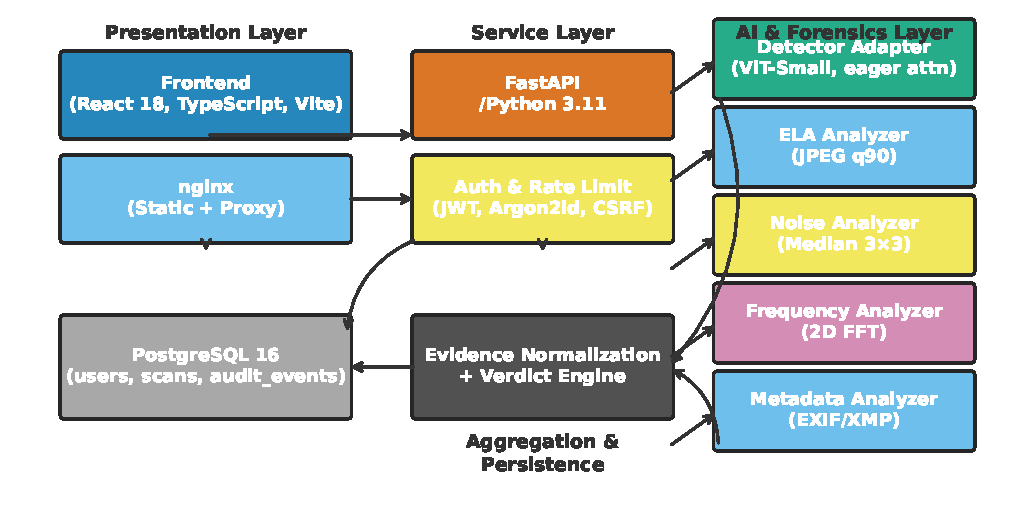
\includegraphics[width=0.95\linewidth]{figures/generated/fig1_architecture.pdf}
  \caption{System architecture: three-tier web application with distinct presentation, service, AI/forensics, and persistence layers. Data flows from upload through parallel forensic analysis to evidence normalization, verdict determination, and persistence.}
  \label{fig:architecture}
\end{figure}

The platform is a three-tier web application (Fig.~\ref{fig:architecture}):

\begin{itemize}
  \item \textbf{Presentation Layer:} Single-page React 18 application (TypeScript 5.x, Vite 5.x, hash-based routing) served via nginx 1.25. No external UI frameworks beyond \texttt{lucide-react} icons. Accessibility: focus-visible outlines, semantic landmarks, reduced-motion respect.
  \item \textbf{Service Layer:} FastAPI 0.110 (Python 3.11) with async SQLAlchemy 2.0 / PostgreSQL 16. Stateless JWT authentication (HS256, Argon2id password hashing via \texttt{argon2-cffi}) delivered as \texttt{HttpOnly, SameSite=Lax} cookies with Bearer header fallback. CSRF origin validation, per-socket-peer login rate limiting (5/min), in-memory sliding-window rate limits for scans (10/min) and default endpoints (120/min).
  \item \textbf{AI \& Forensics Layer:} Detector adapter (thread-safe singleton) loading \texttt{ViTForImageClassification} once per process; four deterministic forensic analyzers (ELA, noise, frequency, metadata) running in parallel; evidence normalization and verdict engine.
  \item \textbf{Persistence Layer:} PostgreSQL 16 with asyncpg. Tables: \texttt{users}, \texttt{scans}, \texttt{audit\_events}. Alembic migrations. Row-level ownership enforced; cross-user access returns 404 (no enumeration). Artifacts stored on filesystem under \texttt{uploads/artifacts/\{scan\_id\}/}.
\end{itemize}

Deployment: Docker Compose (dev) and \texttt{compose.staging.yaml} (TLS termination at \texttt{127.0.0.1:8443} via self-signed certificate, nginx proxy). The staging stack \texttt{pp13} has been live-verified.

\subsection{Evidence Normalization Schema}
\label{sec:evidence-schema}

All detector and forensic outputs are mapped to \texttt{NormalizedEvidenceItem} (Pydantic model) with the following fields:

\begin{table}[t]
\caption{NormalizedEvidenceItem schema fields.}
\label{tab:evidence-schema}
\centering
\begin{tabular}{>{\ttfamily}l p{5.5cm}}
\toprule
Field & Description \\
\midrule
id & Unique identifier (model ID or analyzer ID) \\
source & \texttt{ai\_detector}, \texttt{forensic\_metadata}, \texttt{forensic\_ela}, \texttt{forensic\_noise}, \texttt{forensic\_frequency} \\
method & \texttt{model\_inference}, \texttt{computed}, \texttt{heuristic}, \texttt{verified}, \texttt{unknown} \\
status & \texttt{ok}, \texttt{error}, \texttt{not\_applicable}, \texttt{present}, \texttt{absent} \\
evidence\_category & \texttt{model\_inference}, \texttt{computed\_observation}, \texttt{heuristic}, \texttt{verified\_evidence}, \texttt{unknown\_or\_unavailable} \\
result & Structured payload (probability, statistics, artifact path) \\
interpretation & Human-readable explanation \\
limitations & String list from the producing component \\
artifact & Relative path to generated forensic image (ELA, noise, FFT) \\
\bottomrule
\end{tabular}
\end{table}

This schema enables the frontend to render structured evidence cards instead of raw JSON (raw JSON remains accessible in a collapsible technical-details section).
The \texttt{evidence\_category} field is the critical discriminator: it separates learned inference from deterministic computation, interpretive heuristics, verified provenance, and explicit unavailability.

\subsection{Forensic Analyzers}
\label{sec:analyzers}

\begin{table}[t]
\caption{Forensic analyzers: methods, evidence categories, and status values.}
\label{tab:analyzers}
\centering
\begin{tabular}{lcccc}
\toprule
Analyzer & Method & Evidence Category & Status Values & Key Parameters \\
\midrule
AI Detector (ViT-Small) & model\_inference & model\_inference & ok, error & $\tau_{\mathrm{AI}}=0.80$, $\tau_{\mathrm{real}}=0.20$ \\
Metadata (EXIF/XMP) & computed & computed\_observation & ok, present, absent & — \\
ELA (JPEG recompress q90) & computed & computed\_observation & ok & quality=90 \\
Noise (median-filter residual) & heuristic & heuristic & ok & filter=3$\times$3 \\
Frequency (2D FFT magnitude) & computed & computed\_observation & ok & log-scale + 1e-5 \\
\bottomrule
\end{tabular}
\end{table}

\subsubsection{Metadata Analyzer}
Extracts format, dimensions, color mode, EXIF tags (via \texttt{PIL.ExifTags}), XMP presence, software, datetime.
Reports \texttt{has\_exif} boolean and tag count.
Limitations: absence of EXIF is common in web images and is \emph{not} evidence of AI generation or tampering; metadata timestamps and software tags can be easily stripped or forged.

\subsubsection{Error Level Analysis (ELA)}
Recompresses image in-memory as JPEG quality 90; computes absolute difference; enhances by scaling to full dynamic range.
Reports \texttt{mean\_difference}, \texttt{max\_difference}, \texttt{std\_difference} on raw difference; saves enhanced ELA visualization artifact.
Limitations: ELA is a heuristic visualization tool and cannot independently establish authenticity or prove forgery; high-frequency textures, text, and sharp edges naturally produce higher compression residuals.

\subsubsection{Noise Residual Analysis}
Grayscale conversion; median filter (3$\times$3) subtraction as high-pass noise residual estimate.
Reports \texttt{noise\_mean}, \texttt{noise\_std}, \texttt{noise\_max}; saves normalized noise map artifact.
Limitations: noise residuals are heuristic estimates heavily influenced by image texture, lighting, and compression; AI-generated images often exhibit distinct noise patterns due to diffusion upsampling, but noise consistency alone is not proof of authenticity.

\subsubsection{Frequency Domain Analysis}
Grayscale; 2D FFT with \texttt{fftshift}; log-magnitude spectrum.
Reports \texttt{mean\_magnitude}, \texttt{std\_magnitude}, \texttt{max\_magnitude}; saves normalized spectrum artifact.
Limitations: frequency domain analysis reveals spectral energy distribution but \emph{cannot} identify specific generators or prove authenticity; strong periodic patterns can arise from legitimate sources (scanner grids, screens, regular textures).

\subsection{Explainability}
\label{sec:explainability}

The detector loads with \texttt{attn\_implementation="eager"} to materialize attention tensors.
From the last layer's multi-head attention, we compute a CLS-to-patch attention rollout summary:
mean/max CLS attention and attention entropy over patches.
If tensors are unavailable (SDPA path, non-finite values, or empty), explainability status is \texttt{unavailable} with empty metrics—no fabricated metrics are substituted.
This is \textbf{not} Grad-CAM; it is a CLS-token attention rollout derived from genuine ViT attention weights (Section~\ref{sec:math-explainability}).

\subsection{Authentication, Audit, and Rate Limiting}
\label{sec:auth-audit}

\paragraph{Authentication (Milestone 12).} Argon2id (via \texttt{argon2-cffi}), JWT HS256 with \texttt{exp/iat/iss/sub/role}, 30-min expiry, HttpOnly/SameSite=Lax cookie + Bearer header fallback. Auth fails closed (503) when signing secret absent or $<$32 chars.

\paragraph{Audit (Milestone 14).} Dedicated short-lived session per event; immediate commit; failures logged and swallowed (availability over atomicity). Bounded event types; dynamic strings clamped and charset-normalized. Never stored: passwords, tokens, cookies, image bytes, raw request bodies, EXIF metadata.

\paragraph{Rate Limiting (Milestone 12).} In-memory sliding window, per-process (single uvicorn worker). Keys: bounded prefixes + normalized UUID/IP only. Login 5/min per socket peer; scans 10/min; default 120/min. Distributed deployment would require Redis or gateway-level limiter.

\section{Mathematical Formulation}
\label{sec:math}

This section documents the implemented computations as numbered equations. Every symbol is defined and every equation represents actual code behavior.

\subsection{Detector Score}
\label{sec:math-detector}

The ViT-Small classifier produces a single logit $z \in \mathbb{R}$ for the fake class.
The detector score $s \in [0,1]$ is the sigmoid of $z$:

\begin{equation}
s = \sigma(z) = \frac{1}{1 + \exp(-z)}.
\label{eq:sigmoid}
\end{equation}

\textbf{Critical distinction:} $s$ is a detector score, \emph{not} a calibrated probability.
The model was not calibrated on deployment data; temperature scaling or isotonic regression has not been applied.
The \texttt{ModelOutput} schema explicitly includes limitations: ``Not calibrated on images from this deployment,'' ``Training data may not cover recent generators,'' ``Single-model screening aid only.''

\subsection{Verdict Function}
\label{sec:math-verdict}

Let $s$ be the primary detector's fake probability (Eq.~\ref{eq:sigmoid}).
Let $\tau_{\mathrm{AI}}$ and $\tau_{\mathrm{real}}$ be the configured thresholds (production: $\tau_{\mathrm{AI}}=0.80$, $\tau_{\mathrm{real}}=0.20$; evaluation: $\tau=0.05$).
The base verdict function $V(s)$ is:

\begin{equation}
V(s) =
\begin{cases}
\text{ANALYSIS\_FAILED}, & \text{if primary missing, status $\neq$ ok, or $s$ is null} \\
\text{LIKELY\_AI}, & s \ge \tau_{\mathrm{AI}} \\
\text{LIKELY\_REAL}, & s \le \tau_{\mathrm{real}} \\
\text{INCONCLUSIVE}, & \text{otherwise}
\end{cases}
\label{eq:verdict}
\end{equation}

The risk level $R$ is then determined as:

\begin{equation}
R =
\begin{cases}
\text{UNKNOWN}, & V(s) = \text{ANALYSIS\_FAILED} \\
\text{HIGH}, & V(s) = \text{LIKELY\_AI} \\
\text{LOW}, & V(s) = \text{LIKELY\_REAL} \land H = 0 \\
\text{MODERATE}, & V(s) = \text{LIKELY\_REAL} \land H > 0 \\
\text{MODERATE}, & V(s) = \text{INCONCLUSIVE}
\end{cases}
\label{eq:risk}
\end{equation}

where $H$ is the count of heuristic anomalies detected among forensic evidence items:
\begin{align}
H &= \sum_{i \in \mathcal{E}_{\mathrm{heuristic}}} \mathbb{1}[\text{anomaly}(e_i)] \\
\text{anomaly}(e_i) &=
\begin{cases}
\text{noise\_std} > 25.0, & e_i.\texttt{id} = \texttt{noise} \\
\text{mean\_difference} > 15.0, & e_i.\texttt{id} = \texttt{ela} \\
\text{false}, & \text{otherwise}
\end{cases}
\label{eq:heuristic-anomaly}
\end{align}

Every verdict includes a \texttt{rationale} list (traceable to evidence items) and a fixed \texttt{not\_claimed} list:
\begin{verbatim}
["generator identity",
 "legal authenticity",
 "localized forgery without verified provenance",
 "calibrated real-world criminal fraud probability"]
\end{verbatim}

\subsection{Error Level Analysis}
\label{sec:math-ela}

Let $I$ be the original image and $J_q$ the JPEG recompression at quality $q=90$.
The difference image $D_q$ is:

\begin{equation}
D_q(x,y,c) = |I(x,y,c) - J_q(x,y,c)|,
\quad (x,y) \in [1..W] \times [1..H], \; c \in \{R,G,B\}.
\label{eq:ela-diff}
\end{equation}

The visualization $E_q$ scales $D_q$ to the full dynamic range:

\begin{equation}
E_q = \frac{255}{\max_{x,y,c} D_q(x,y,c)} \cdot D_q,
\label{eq:ela-scale}
\end{equation}

with the convention $\max D_q = 1$ if all differences are zero.
The reported statistics are computed on the raw difference $D_q$:
$\texttt{mean\_difference} = \mathbb{E}[D_q]$, $\texttt{std\_difference} = \sqrt{\mathrm{Var}[D_q]}$, $\texttt{max\_difference} = \max D_q$.

\subsection{Frequency Analysis}
\label{sec:math-frequency}

Let $I_g$ be the grayscale conversion of $I$.
The 2D discrete Fourier transform is:

\begin{equation}
F(u,v) = \sum_{x=0}^{M-1} \sum_{y=0}^{N-1}
I_g(x,y) \exp\!\left[-j2\pi\left(\frac{ux}{M}+\frac{vy}{N}\right)\right],
\label{eq:fft}
\end{equation}

with zero-frequency shift: $F_{\mathrm{shift}} = \mathrm{fftshift}(F)$.
The log-magnitude spectrum for visualization is:

\begin{equation}
S(u,v) = 20 \log\!\big(|F_{\mathrm{shift}}(u,v)| + 10^{-5}\big).
\label{eq:log-magnitude}
\end{equation}

Reported statistics: $\texttt{mean\_magnitude} = \mathbb{E}[S]$, $\texttt{std\_magnitude} = \sqrt{\mathrm{Var}[S]}$, $\texttt{max\_magnitude} = \max S$.

\subsection{Noise Residual}
\label{sec:math-noise}

Let $\mathcal{M}_k$ denote the median filter with kernel size $k=3$.
The noise residual $R$ is:

\begin{equation}
R(x,y) = I_g(x,y) - \mathcal{M}_3(I_g)(x,y).
\label{eq:noise-residual}
\end{equation}

Reported statistics: $\texttt{noise\_mean} = \mathbb{E}[R]$, $\texttt{noise\_std} = \sqrt{\mathrm{Var}[R]}$, $\texttt{noise\_max} = \max |R|$.
The visualization normalizes $|R|$ to $[0, 255]$.

\subsection{Classification Metrics}
\label{sec:math-metrics}

Let $TP$, $TN$, $FP$, $FN$ denote confusion-matrix counts with positive class = AI-generated.
The standard metrics are:

\begin{align}
\operatorname{Accuracy} &= \frac{TP + TN}{TP + TN + FP + FN} \\
\operatorname{Precision} &= \frac{TP}{TP + FP} \\
\operatorname{Recall} &= \frac{TP}{TP + FN} \\
F_1 &= \frac{2 \cdot \operatorname{Precision} \cdot \operatorname{Recall}}{\operatorname{Precision} + \operatorname{Recall}} \\
\operatorname{FPR} &= \frac{FP}{FP + TN} \\
\operatorname{FNR} &= \frac{FN}{FN + TP} \\
\operatorname{Specificity} &= \frac{TN}{TN + FP} \\
\operatorname{Balanced~Accuracy} &= \frac{\operatorname{Recall} + \operatorname{Specificity}}{2}
\label{eq:metrics}
\end{align}

ROC-AUC and PR-AUC are computed from the continuous scores using the trapezoidal rule.

\subsection{Balanced Accuracy and Threshold Selection}
\label{sec:math-threshold}

The validation threshold selection maximizes balanced accuracy:

\begin{equation}
\tau^* = \arg\max_{\tau \in \mathcal{T}} \operatorname{BA}(\tau),
\qquad \operatorname{BA}(\tau) = \frac{\operatorname{TPR}(\tau) + \operatorname{TNR}(\tau)}{2},
\label{eq:ba}
\end{equation}

where $\mathcal{T} = \{0.05, 0.10, \dots, 0.95\}$.
The selected threshold $\tau^* = 0.05$ was then frozen and applied once to the locked test split.

\subsection{Confidence Intervals}
\label{sec:math-ci}

The 95\% confidence interval for accuracy uses the normal approximation:

\begin{equation}
\operatorname{CI}_{95} = \hat{p} \pm 1.96 \sqrt{\frac{\hat{p}(1-\hat{p})}{n}},
\qquad \hat{p} = \operatorname{Accuracy},
\label{eq:ci}
\end{equation}

where $n$ is the test sample count. This assumes independent Bernoulli trials; the interval is reported for accuracy only.

\subsection{Evidence Representation}
\label{sec:math-evidence}

A normalized evidence item is a tuple:

\begin{equation}
e = \langle \texttt{id}, \texttt{source}, \texttt{method}, \texttt{status},
\texttt{category}, \texttt{result}, \texttt{interpretation}, \texttt{limitations}, \texttt{artifact} \rangle,
\label{eq:evidence}
\end{equation}

where $\texttt{category} \in \{\texttt{model\_inference}, \texttt{computed\_observation},
\texttt{heuristic}, \texttt{verified\_evidence}, \texttt{unknown\_or\_unavailable}\}$.
The assessment is the set $\mathcal{E} = \{e_1, \dots, e_k\}$ with one detector item and one per forensic analyzer.

\subsection{Explainability: Attention Rollout}
\label{sec:math-explainability}

Let $\mathbf{A}^{(\ell)} \in \mathbb{R}^{h \times L \times L}$ be the attention tensor for layer $\ell$ ($h$ heads, sequence length $L$).
Using the last layer $\ell = \mathcal{L}$ (12 for ViT-Small), the mean head attention is:

\begin{equation}
\bar{\mathbf{A}} = \frac{1}{h} \sum_{i=1}^h \mathbf{A}^{(\mathcal{L})}_i \in \mathbb{R}^{L \times L}.
\label{eq:mean-head}
\end{equation}

The CLS-to-patch attention vector is the first row excluding the CLS self-attention:

\begin{equation}
\mathbf{a}_{\mathrm{CLS}} = \bar{\mathbf{A}}[0, 1:] \in \mathbb{R}^{L-1}.
\label{eq:cls-patches}
\end{equation}

Normalized to a probability distribution:

\begin{equation}
\mathbf{p} = \frac{\mathbf{a}_{\mathrm{CLS}}}{\sum_j a_{\mathrm{CLS},j} + 10^{-12}}.
\label{eq:cls-probs}
\end{equation}

Reported metrics:
\begin{align}
\texttt{num\_layers} &= \mathcal{L}, \\
\texttt{num\_heads} &= h, \\
\texttt{num\_patches} &= L-1, \\
\texttt{mean\_cls\_attention} &= \mathbb{E}[\mathbf{p}], \\
\texttt{max\_cls\_attention} &= \max \mathbf{p}, \\
\texttt{attention\_entropy} &= -\sum_j p_j \log(p_j + 10^{-12}).
\label{eq:attn-metrics}
\end{align}

If any tensor is unavailable, non-finite, or empty, the entire explainability object is \texttt{unavailable} with empty metrics.

\section{Implementation}
\label{sec:implementation}

\subsection{Detector Adapter}
\label{sec:detector-impl}

\texttt{DetectorAdapter} is a thread-safe singleton loading \texttt{ViTForImageClassification} and \texttt{ViTImageProcessor} once per process.
Device selection: \texttt{auto} tries CUDA then CPU; \texttt{cpu} or \texttt{cuda} forces device.
Inference runs with \texttt{torch.inference\_mode()}, \texttt{output\_attentions=True}.
Logit $\to$ sigmoid $\to$ \texttt{fake\_probability} $\in [0,1]$ (Eq.~\ref{eq:sigmoid}).
Latency measured with \texttt{torch.cuda.synchronize()} on GPU.
Health endpoint reports \texttt{detector\_loaded}, \texttt{cuda\_available}, \texttt{gpu\_name}, \texttt{load\_error}.

Configuration (pinned):
\begin{verbatim}
model_id = "buildborderless/CommunityForensics-DeepfakeDet-ViT"
model_revision = "ac6ee457bea904a373065754107451793b56db00"
expected_num_labels = 1
expected_shortest_edge = 440
expected_crop = 384
attn_implementation = "eager"
\end{verbatim}
Config mismatch raises \texttt{ConfigMismatchError} at load time.

\subsection{Scan Pipeline}
\label{sec:scan-pipeline}

\begin{figure}[t]
  \centering
  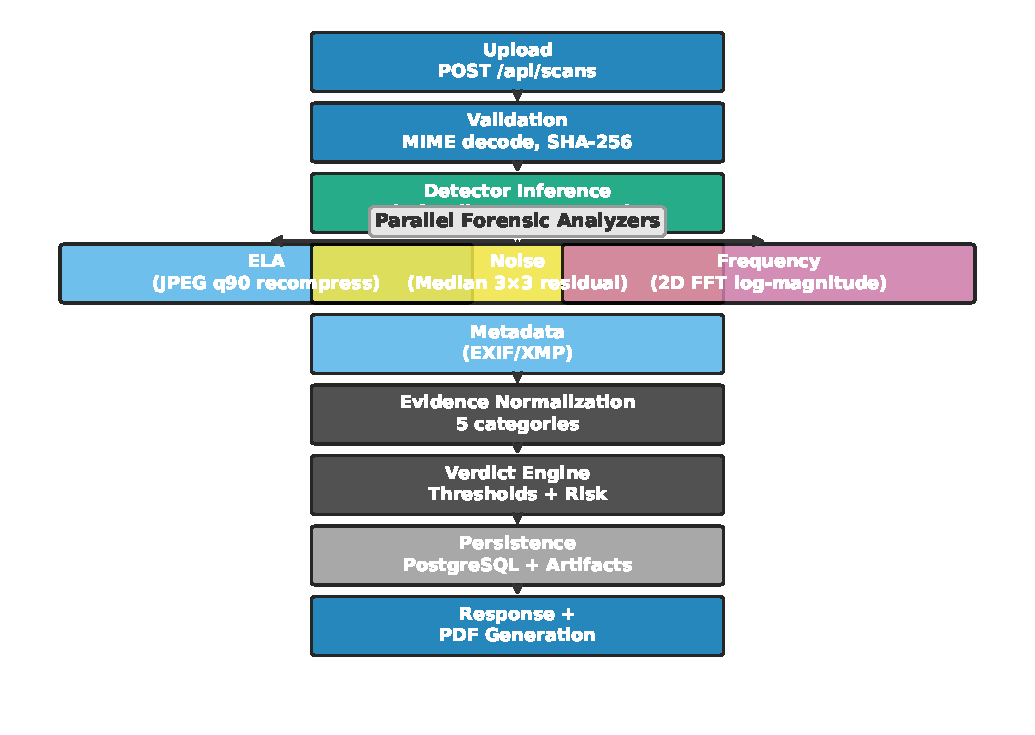
\includegraphics[width=0.95\linewidth]{figures/generated/fig2_pipeline.pdf}
  \caption{Scan processing pipeline: validation $\to$ parallel detector + forensic analysis $\to$ evidence normalization $\to$ verdict $\to$ persistence $\to$ response/PDF.}
  \label{fig:pipeline}
\end{figure}

The pipeline (Fig.~\ref{fig:pipeline}) executes:
\begin{enumerate}
  \item \texttt{POST /api/scans} (authenticated, CSRF, rate-limited).
  \item Validate MIME via decode (not header); decode via \texttt{PIL}; compute SHA-256.
  \item Run detector inference $\to$ \texttt{ModelOutput} (Eq.~\ref{eq:sigmoid}).
  \item Run all forensic analyzers in parallel $\to$ \texttt{Indicator} list (Eqs.~\ref{eq:ela-diff}--\ref{eq:noise-residual}).
  \item \texttt{normalize\_evidence} $\to$ unified schema (Eq.~\ref{eq:evidence}, Table~\ref{tab:evidence-schema}).
  \item \texttt{aggregate\_assessment} $\to$ verdict + risk (Eqs.~\ref{eq:verdict}--\ref{eq:heuristic-anomaly}) + summary.
  \item Persist \texttt{Scan} row with full \texttt{full\_result} JSON.
  \item Return \texttt{ScanCreateResponse} with \texttt{scan\_id}, \texttt{status}, \texttt{result}.
\end{enumerate}

Database errors during persistence are logged but do not fabricate success; the computed result is still returned to the client.

\subsection{Frontend Architecture}
\label{sec:frontend}

Single-file \texttt{App.tsx} (1,431 lines) with hash-based routing (\texttt{\#landing}, \texttt{\#login}, \texttt{\#dashboard}, \texttt{\#upload}, \texttt{\#history}, \texttt{\#scan-\{id\}}).
Views: Landing, Login, Dashboard, Upload (drag-drop, preview), Results (verdict band, evidence cards, metadata table, artifact gallery, technical-details collapsible), Archive (scan list), PDF download.
Internal \texttt{PhoenixMascot} SVG component with states: \texttt{idle}, \texttt{investigating}, \texttt{reassuring}.
Design tokens in \texttt{index.css}: monospace typography, \texttt{.bg-*} background classes, amber primary CTA, CSS keyframe animations only.

\subsection{PDF Report Generation}
\label{sec:pdf}

\texttt{report.py} uses ReportLab \texttt{platypus} to generate a multi-page PDF dossier containing:
scan metadata, input details, verdict/risk/rationale, model output, forensic indicator results, evidence items, explainability metrics, and embedded artifact images (ELA, noise, FFT).
Served via \texttt{GET /api/scans/\{scan\_id\}/report.pdf} (authenticated).

\section{Evaluation Methodology and Results}
\label{sec:evaluation}

\subsection{Dataset Construction}
\label{sec:dataset}

The PHANTOM PHOENIX evaluation manifest (\texttt{datasets/manifests/dataset\_manifest.csv}) contains 6,000 images (3,000 real, 3,000 AI-generated) sourced from OpenFake \texttt{core} configuration.
Stratified random sampling by \texttt{(label, generator\_family)} with fixed seed 42 yielded:

\begin{table}[t]
\caption{Dataset split distribution (verified zero SHA-256 duplicates, zero missing/corrupt files).}
\label{tab:splits}
\centering
\begin{tabular}{lccc}
\toprule
Split & Real & AI-Generated & Total \\
\midrule
Train & 2,099 & 2,089 & 4,188 \\
Validation & 449 & 441 & 890 \\
Test & 452 & 470 & 922 \\
\bottomrule
\end{tabular}
\end{table}

Test-set AI generator families: \texttt{z-image-turbo} (128), \texttt{flux.2-klein-9b} (85), \texttt{illustrious} (61), \texttt{gpt-image-1.5} (59), \texttt{midjourney-7} (34), \texttt{veo-3} (21), \texttt{wan-video-2.5} (13), and 13 minor families ($n \le 10$).
Real test sources: ImageNet (304), DOCCI (148) — distinct from training real sources (LAION, Pexels).

\begin{figure}[t]
  \centering
  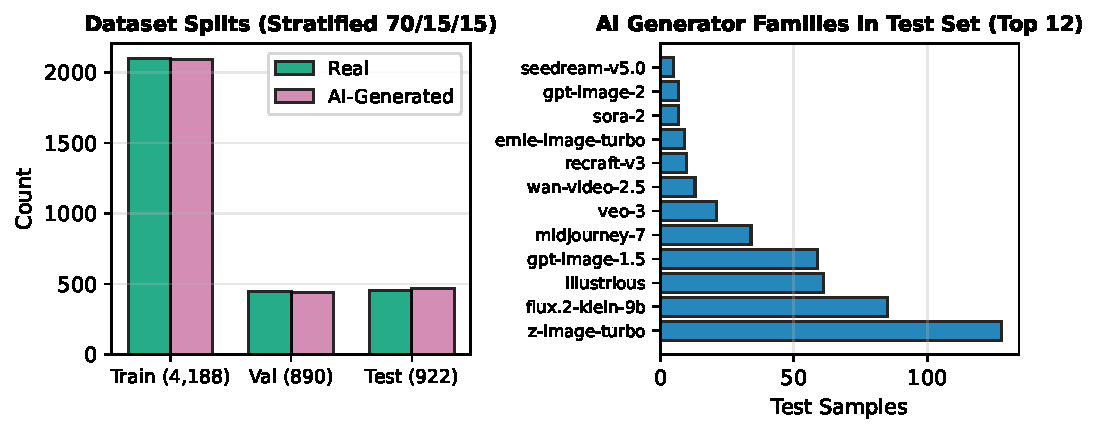
\includegraphics[width=0.95\linewidth]{figures/generated/fig9_dataset.pdf}
  \caption{Dataset composition: (left) stratified split counts; (right) AI generator families in test set. Minor families ($n \le 10$) appear in both train and test splits.}
  \label{fig:dataset}
\end{figure}

\subsection{Evaluation Protocol}
\label{sec:eval-protocol}

\paragraph{Model \& Preprocessing.}
\texttt{buildborderless/CommunityForensics-DeepfakeDet-ViT} @ revision \texttt{ac6ee457bea904a373065754107451793b56db00}, \texttt{attn\_implementation="eager"}.
ViTImageProcessor: shortest edge 440, center crop 384, CLIP normalization.

\paragraph{Threshold Selection (Validation).}
Swept thresholds 0.05–0.95 on validation split (890 samples).
Selected threshold maximizing balanced accuracy (Eq.~\ref{eq:ba}): \textbf{0.05}.
Validation at 0.05: accuracy 0.7258, precision 0.9758, recall 0.4580, F1 0.6235, FPR 0.0111, BA 0.7235.

\paragraph{Frozen Test Evaluation.}
The selected threshold (0.05) was applied \emph{once} to the locked test split (922 samples) without further tuning.

\subsection{Results}
\label{sec:results}

\begin{table}[t]
\caption{Locked test-set evaluation (922 samples, threshold 0.05). CI: 95\% normal approximation for accuracy (Eq.~\ref{eq:ci}).}
\label{tab:test-results}
\centering
\begin{tabular}{lc}
\toprule
Metric & Value \\
\midrule
Accuracy & 0.7538 [0.7260, 0.7816] \\
Precision (AI) & 0.9765 \\
Recall (AI) & 0.5298 \\
F1 Score (AI) & 0.6869 \\
ROC-AUC & 0.8959 \\
PR-AUC & 0.9163 (threshold-independent) \\
False Positive Rate & 0.0133 (6 / 452) \\
False Negative Rate & 0.4702 (221 / 470) \\
Balanced Accuracy & 0.7583 \\
Confusion Matrix & [[446, 6], [221, 249]] \\
\bottomrule
\end{tabular}
\end{table}

\begin{figure}[t]
  \centering
  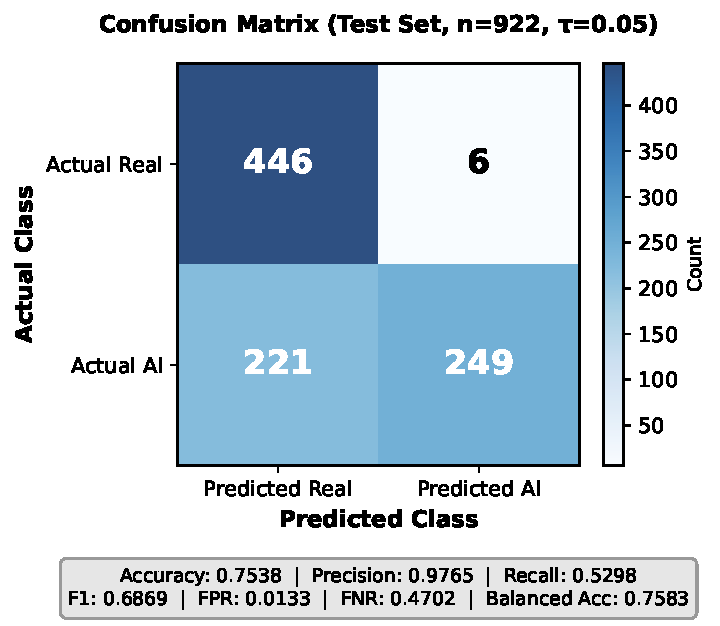
\includegraphics[width=0.95\linewidth]{figures/generated/fig6_confusion_matrix.pdf}
  \caption{Confusion matrix on locked test set (n=922, $\tau=0.05$). Rows = actual, columns = predicted. Positive class = AI-generated.}
  \label{fig:confusion}
\end{figure}

\begin{table}[t]
\caption{Threshold comparison on locked test set (922 samples). Production thresholds ($\tau_{\mathrm{AI}}=0.80$, $\tau_{\mathrm{real}}=0.20$) prioritize screening conservativeness; evaluation threshold ($\tau=0.05$) maximizes validation balanced accuracy.}
\label{tab:threshold-comp}
\centering
\begin{tabular}{lcccccc}
\toprule
Threshold & Accuracy & Precision & Recall & F1 & FPR & FNR \\
\midrule
0.50 (baseline) & 0.6562 & 0.9935 & 0.3277 & 0.4928 & 0.0022 & 0.6723 \\
0.20 (candidate) & 0.6941 & 0.9845 & 0.4064 & 0.5753 & 0.0066 & 0.5936 \\
0.05 (selected) & \textbf{0.7538} & \textbf{0.9765} & \textbf{0.5298} & \textbf{0.6869} & 0.0133 & 0.4702 \\
\bottomrule
\end{tabular}
\end{table}

\begin{figure}[t]
  \centering
  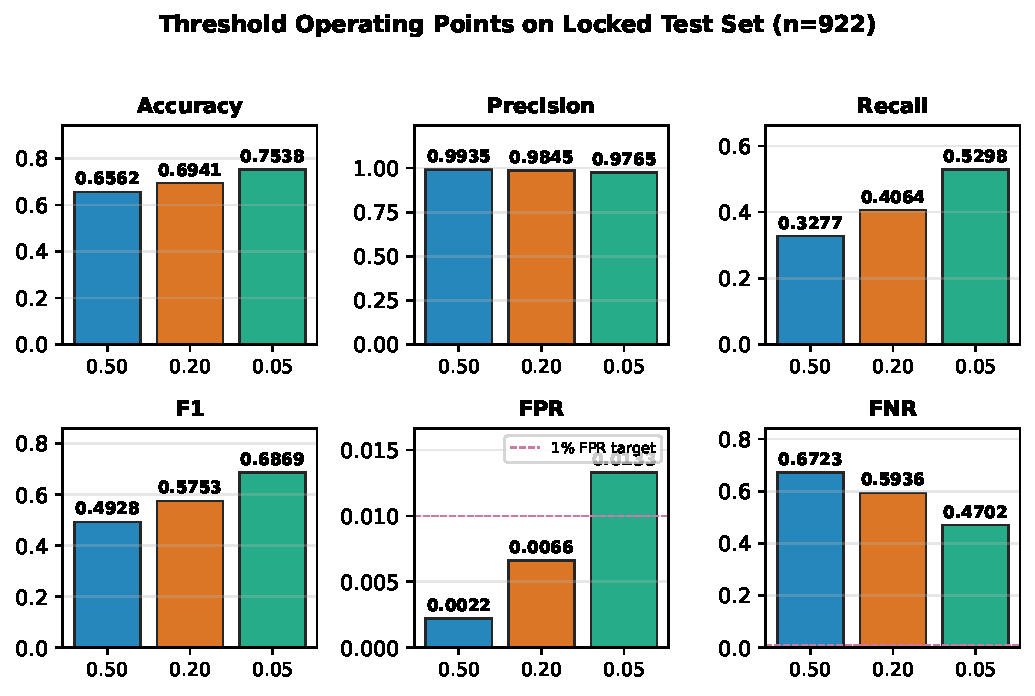
\includegraphics[width=0.95\linewidth]{figures/generated/fig7_thresholds.pdf}
  \caption{Threshold operating points on locked test set. Lower threshold increases recall but also FPR; the 1\% FPR target line marks the operational constraint.}
  \label{fig:thresholds}
\end{figure}

The selected threshold (0.05) increases AI recall from 32.77\% to 52.98\% while maintaining FPR at 1.33\% (6 false positives on 452 real images).
Production thresholds (0.80 / 0.20) are distinct from evaluation thresholds and prioritize screening conservativeness.

\begin{figure}[t]
  \centering
  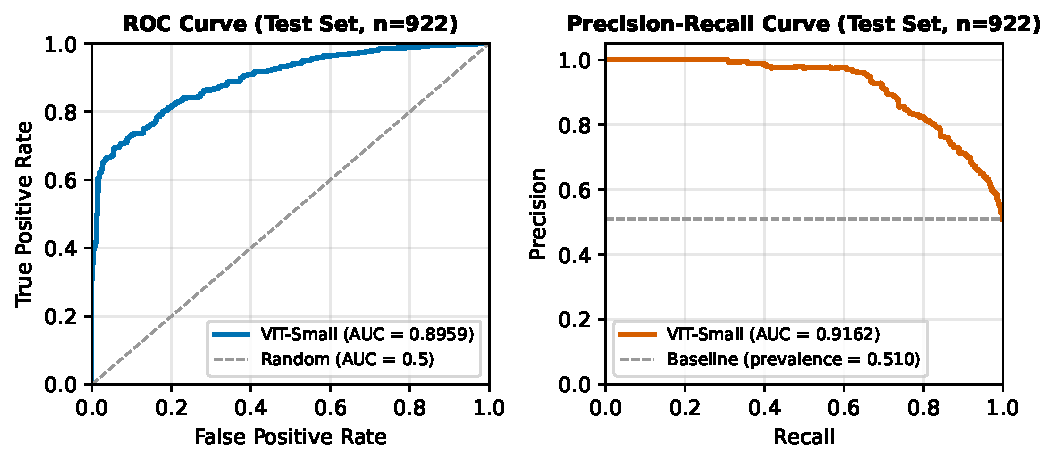
\includegraphics[width=0.95\linewidth]{figures/generated/fig8_roc_pr.pdf}
  \caption{ROC and Precision-Recall curves computed from per-image scores on the locked test set (n=922). ROC-AUC = 0.8959, PR-AUC = 0.9163. Baseline = class prevalence (0.510).}
  \label{fig:roc-pr}
\end{figure}

\begin{figure}[t]
  \centering
  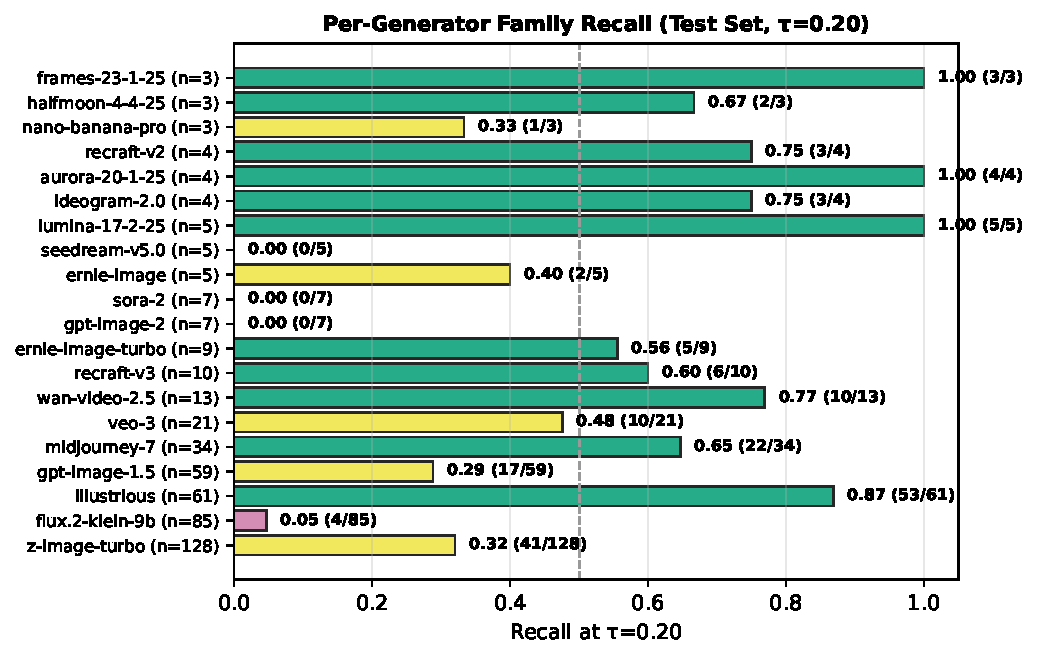
\includegraphics[width=0.95\linewidth]{figures/generated/fig12_per_family.pdf}
  \caption{Per-generator family recall at $\tau=0.20$ on test set. Families with $n < 5$ are marked; true unseen-generator generalization requires holding out entire major families.}
  \label{fig:per-family}
\end{figure}

\paragraph{Inference Latency.}
On CPU (deployment environment): mean 39.7 ms, median 27.5 ms, total 36.6 s for 922 images (batch size 1).

\begin{figure}[t]
  \centering
  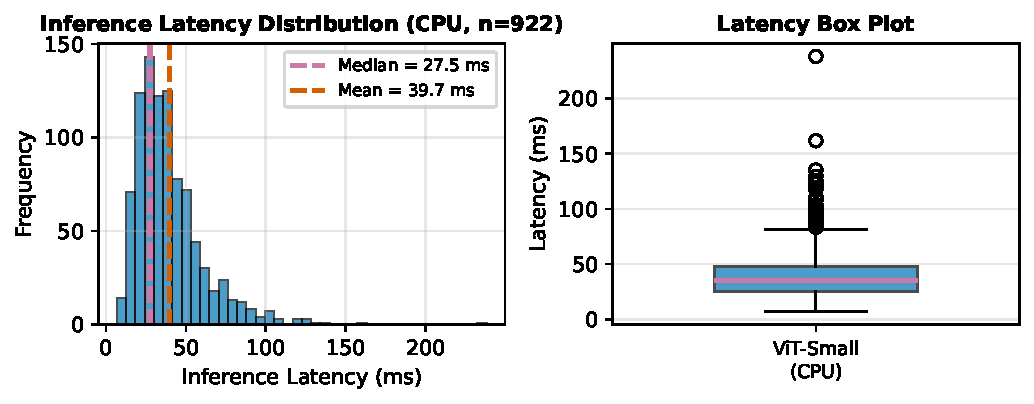
\includegraphics[width=0.95\linewidth]{figures/generated/fig11_latency.pdf}
  \caption{Inference latency distribution (CPU, n=922). Mean = 39.7 ms, median = 27.5 ms. Log-normal shape characteristic of transformer inference on CPU.}
  \label{fig:latency}
\end{figure}

\paragraph{System Verification Tests.}
Frontend: TypeScript strict build (0 errors), Vite production build (279 kB JS, 82 kB gzip), oxlint (5 pre-existing warnings), Playwright E2E smoke (4/4 passed: landing gate, hash routing, protected redirect, generic login failure).
Backend: 156 unit tests pass (166 with DB). PostgreSQL integration tests not re-run against the valued \texttt{pp13} database (fixture deletes scan rows).
Docker Compose config valid; \texttt{git diff --check} clean.

\subsection{Dataset Confounding (E2 Experiment)}
\label{sec:confounding}

\begin{figure}[t]
  \centering
  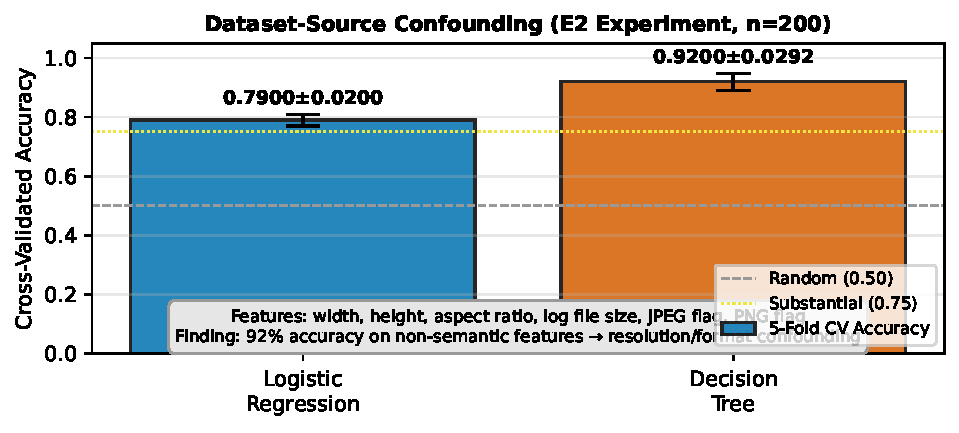
\includegraphics[width=0.95\linewidth]{figures/generated/fig10_confounding.pdf}
  \caption{Format-only classifier (6 non-semantic features: width, height, aspect ratio, log file size, JPEG flag, PNG flag) achieves 92\% CV accuracy on 200-image subset, demonstrating measurable dataset-source confounding.}
  \label{fig:confounding}
\end{figure}

As documented in the E2 Decision Report~\cite{experiment-e2-decision}, a format-only diagnostic classifier (Logistic Regression and Decision Tree) using 6 non-semantic features achieved 92\% cross-validated accuracy on a 200-image subset.
This indicates that generator default resolutions (e.g., 1024$\times$1024, 384$\times$384) create shortcut features that a detector could exploit.
While the full 6,000-image manifest is stratified by generator family, minor families ($n < 5$) appear in both train and test splits; true unseen-generator generalization requires holding out entire major families (not done).
Cryptographic SHA-256 deduplication does not detect near-duplicate or semantically related images.

\section{Case Walkthrough}
\label{sec:walkthrough}

\begin{enumerate}
  \item \textbf{Landing.} User arrives at \texttt{https://host/\#landing}; clicks \texttt{Investigator Dashboard} $\to$ routed to sign-in (Fig.~\ref{fig:landing}).
  \item \textbf{Authentication.} Credentials submitted to \texttt{POST /api/auth/login}; HttpOnly JWT cookie set; redirected to \texttt{\#dashboard} (Fig.~\ref{fig:dash-upload} left).
  \item \textbf{Upload.} User drags \texttt{real\_000002.jpg} (900$\times$700 PNG, 93 KB); preview renders; submits (Fig.~\ref{fig:dash-upload} right).
  \item \textbf{Inference.} Backend validates, decodes, runs ViT-Small detector ($\sim$40 ms), four forensic analyzers, aggregates evidence, determines verdict, persists scan.
  \item \textbf{Results.} Browser navigates to \texttt{\#scan-\{id\}}; renders verdict, score, evidence cards, metadata table, artifact gallery (Fig.~\ref{fig:results}, \ref{fig:artifacts}). Raw JSON available in collapsible \texttt{Technical Details}.
  \item \textbf{PDF.} User clicks \texttt{Download PDF Report} $\to$ \texttt{GET /api/scans/\{id\}/report.pdf} returns 400 KB \texttt{application/pdf} (\%PDF-1.4).
  \item \textbf{Archive.} User visits \texttt{\#history} $\to$ paginated scan list from \texttt{GET /api/scans}.
  \item \textbf{Logout.} Session cookie cleared; subsequent \texttt{/api/auth/me} returns 401; user routed to \texttt{\#login}.
\end{enumerate}
All steps verified against the running \texttt{pp13} staging stack.

\begin{figure}[t]
  \centering
  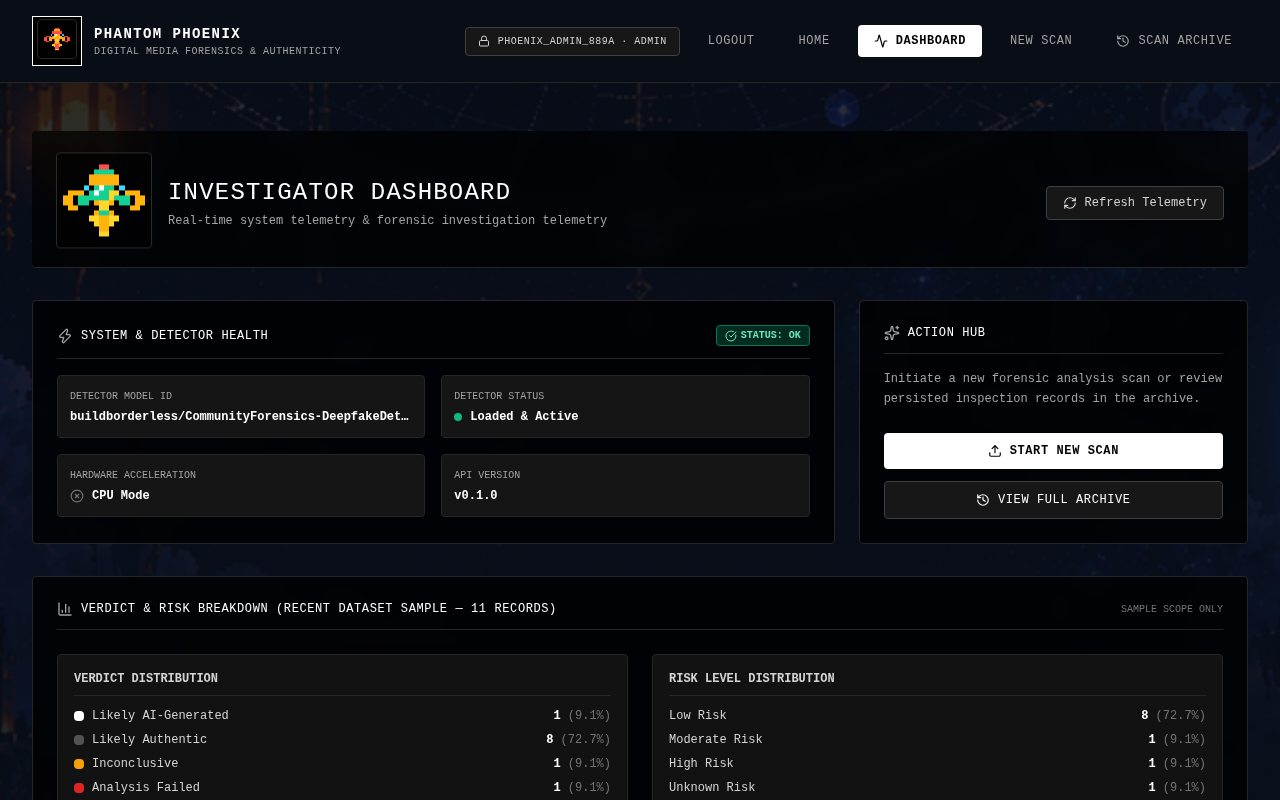
\includegraphics[width=0.48\linewidth]{figures/03-dashboard.png}
  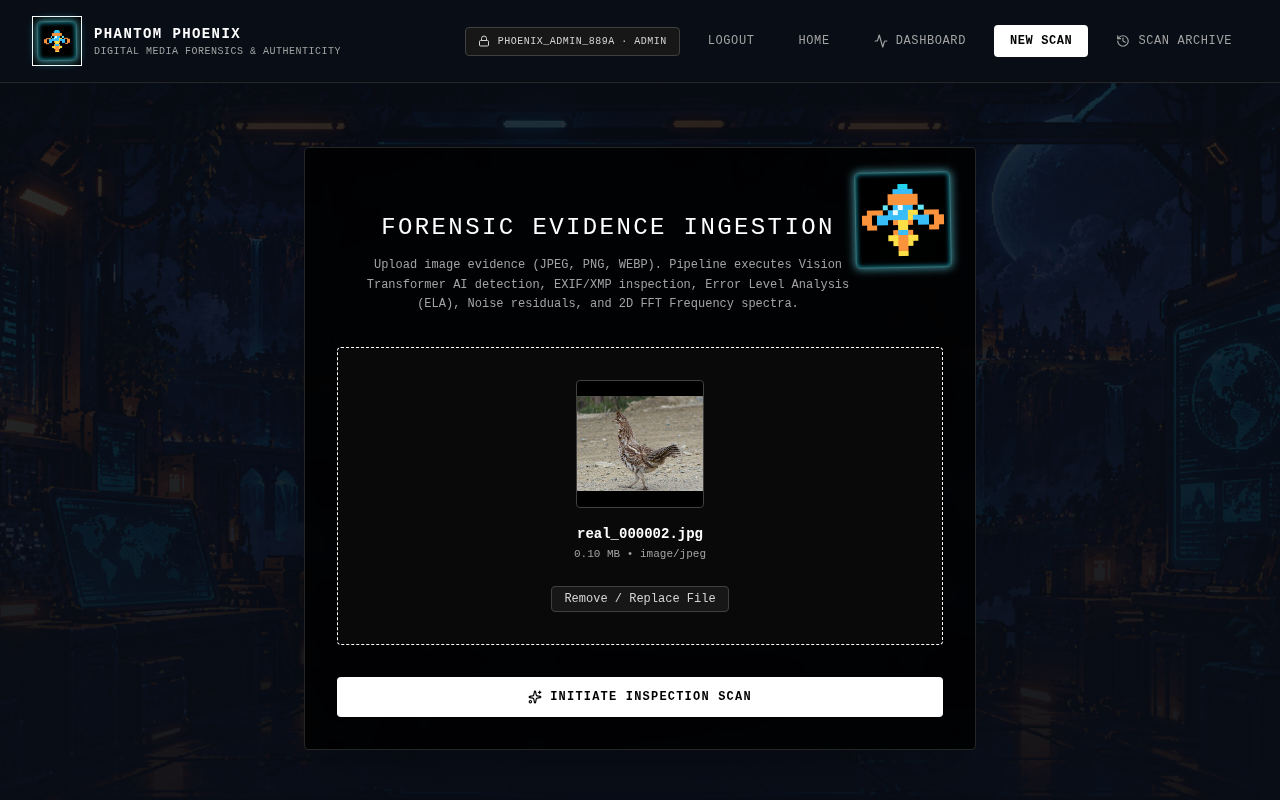
\includegraphics[width=0.48\linewidth]{figures/04-upload.png}
  \caption{Investigator dashboard (left) and upload view with real-image preview (right).}
  \label{fig:dash-upload}
\end{figure}

\begin{figure}[t]
  \centering
  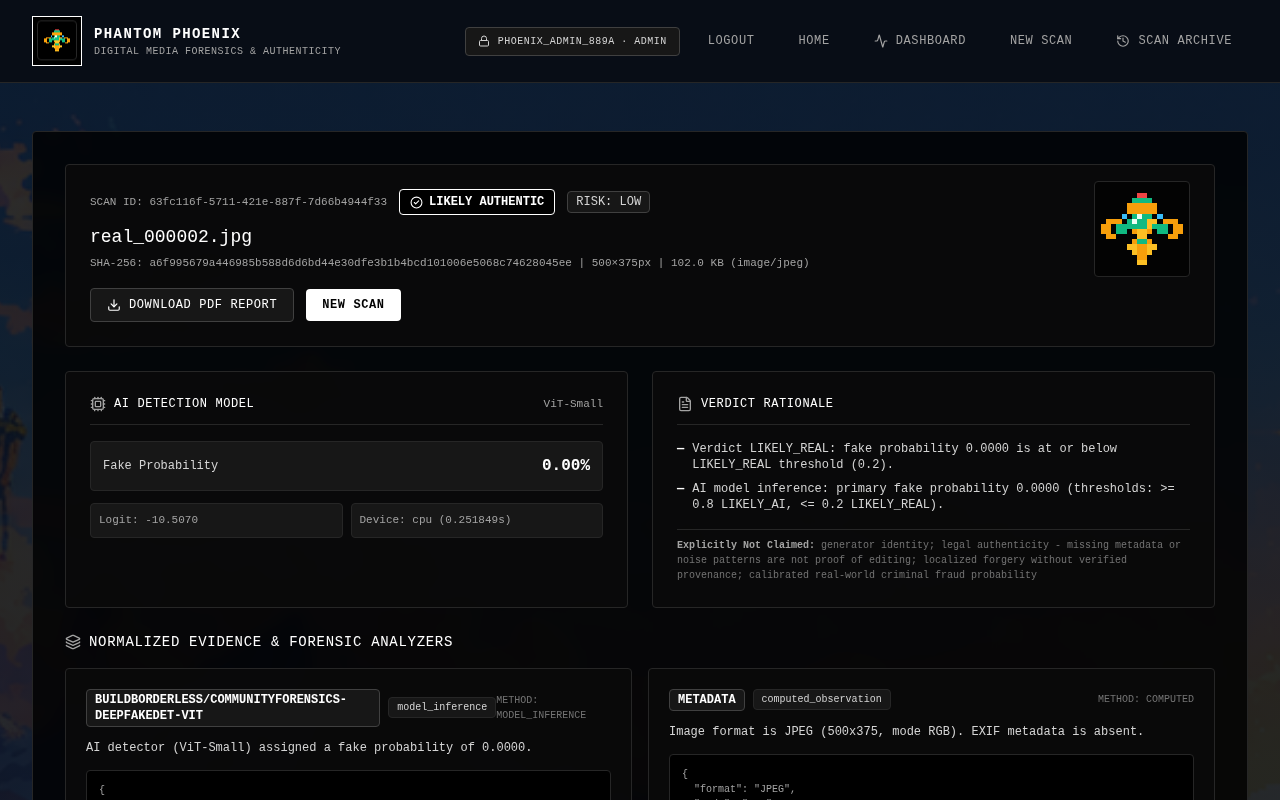
\includegraphics[width=0.95\linewidth]{figures/05-results-overview.png}
  \caption{Results overview: verdict band (LIKELY\_REAL), forensic score, structured evidence cards replacing raw JSON.}
  \label{fig:results}
\end{figure}

\begin{figure}[t]
  \centering
  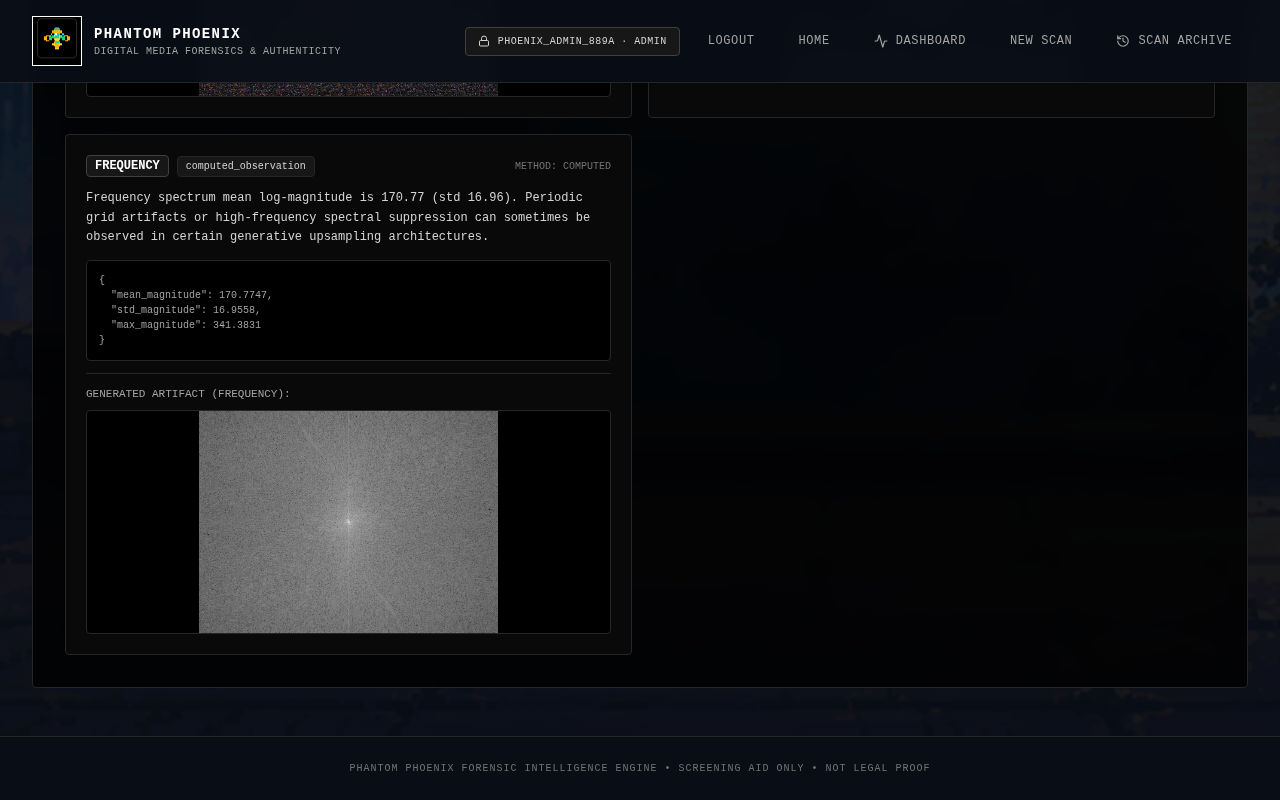
\includegraphics[width=0.48\linewidth]{figures/06-metadata-evidence.png}
  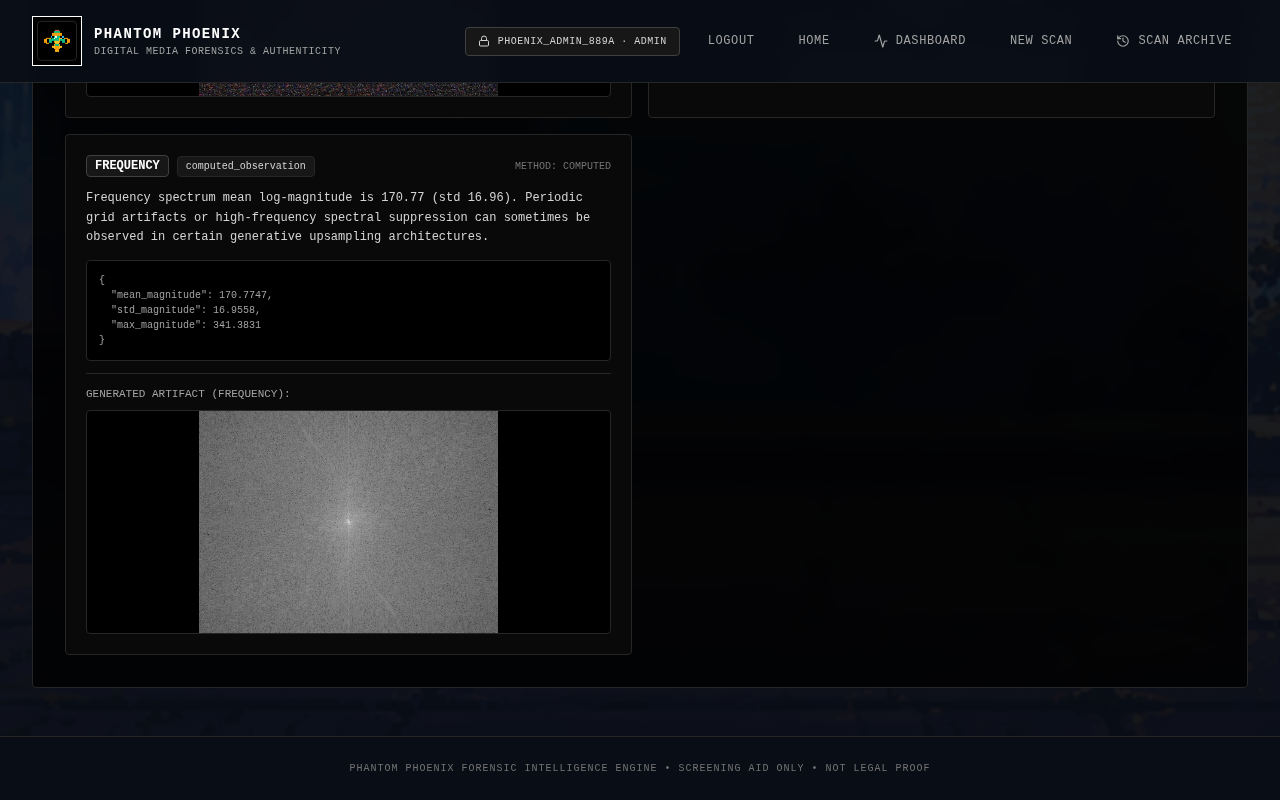
\includegraphics[width=0.48\linewidth]{figures/07-forensic-artifacts.png}
  \caption{Metadata \& evidence detail (left) and forensic artifact gallery (ELA, noise, FFT) (right). Artifacts served via authenticated \texttt{/api/artifacts/} endpoints.}
  \label{fig:artifacts}
\end{figure}

\begin{figure}[t]
  \centering
  
\includegraphics[width=0.48\linewidth]{figures/01-landing.png}
  \caption{Landing page with phoenix mascot and amber primary CTA.}
  \label{fig:landing}
\end{figure}

\section{Limitedations, Threats to Validity, and Ethical Considerations}
\label{sec:limitations}

\subsection{Dataset and Evaluation Limitations}
\begin{itemize}
  \item The 6,000-image manifest derives from OpenFake \texttt{core} v1; generator-family labels reflect provider metadata and may contain misattributions.
  \item Minor generator families ($n < 5$) appear in both train and test splits; true unseen-generator generalization requires holding out entire major families (not done).
  \item Resolution/format confounding exists: Decision Tree on 6 non-semantic features achieves 92\% CV accuracy on 200-image subset (Fig.~\ref{fig:confounding}), indicating measurable dataset-source shortcut features~\cite{experiment-e2-decision}.
  \item The validation threshold selection (maximizing balanced accuracy at 0.05) was performed on the same validation split used for hyperparameter awareness; the test evaluation is frozen but the selection criterion itself is not independently validated on a third hold-out set.
  \item Historical pilot metrics (50-image OpenFake pilot, accuracy 0.62, recall 0.24 at 0.50) are reported in \texttt{PHASE2\_PILOT\_ERROR\_ANALYSIS.md} but are not representative of the full 922-sample test evaluation.
  \item No ablation study isolates the contribution of forensic analyzers to verdict accuracy; evidence fusion improvement claims are not substantiated by controlled baselines.
\end{itemize}

\subsection{System Limitations}
\begin{itemize}
  \item Single-worker in-memory rate limiting; horizontal scaling requires Redis/gateway.
  \item JWT tokens are snapshots; account disable/role revocation takes effect at token expiry ($\le$30 min); no server-side session store or denylist.
  \item Audit trail is not a tamper-proof ledger (DB admin can modify); availability prioritized over forced atomicity.
  \item Explainability is attention rollout (Eqs.~\ref{eq:mean-head}--\ref{eq:attn-metrics}), not gradient-based (Grad-CAM); may not localize generator-specific artifacts.
  \item Production thresholds (0.80/0.20) are provisional screening defaults, not calibrated probabilities.
  \item Image-only; no video, audio, or multimodal analysis.
\end{itemize}

\subsection{Ethical Considerations}
\begin{itemize}
  \item The platform is a \emph{screening aid}, not a forensic proof system. Mandatory \texttt{not\_claimed} disclaimers are part of every verdict.
  \item False positives (real images flagged as AI) carry reputational and evidentiary risk; production threshold 0.80 minimizes this at the cost of recall.
  \item No biometric data processed; EXIF/XMP stripped from stored artifacts; no PII in audit logs.
  \item Model trained on Community Forensics dataset (CC-BY-NC-4.0 subsets); deployment respects license terms.
\end{itemize}

\section{Conclusion and Future Work}
\label{sec:conclusion}

\textsc{Phantom Phoenix} delivers a complete, auditable forensic screening pipeline: ViT-Small detector (Community Forensics), classical forensic analyzers, normalized evidence schema, deterministic verdict engine, authenticated persistence, audit logging, and PDF dossiers.
On the locked 922-sample test split, the frozen validation-selected threshold achieves 75.38\% accuracy, 52.98\% AI recall, 1.33\% FPR, and 0.8959 ROC-AUC.

Future work:
\begin{itemize}
  \item Calibrated probability outputs (temperature scaling, isotonic regression) to replace provisional thresholds.
  \item Unseen-generator hold-out evaluation (entire major families withheld from training).
  \item Ablation studies quantifying forensic analyzer contribution to verdict accuracy.
  \item Gradient-based explainability (Integrated Gradients, attention-flow) with artifact generation.
  \item Multi-modal extension: video frame analysis, audio-visual consistency.
  \item Distributed rate limiting and audit hardening for multi-replica deployments.
  \item Formal red-team evaluation of adversarial robustness.
\end{itemize}

\section*{Acknowledgment}
This work was carried out under the guidance of Dr. Soumya K N at Jyothy Institute of Technology, Bengaluru.
We acknowledge the Community Forensics authors (Park \& Owens, CVPR 2025) and OpenFake authors (Livernoche et al., arXiv 2025) for open datasets and models.

\bibliographystyle{IEEEtran}
\bibliography{references}

\end{document}